%\documentclass[12pt,handout]{beamer}
\documentclass{beamer}
\usepackage[ngerman]{babel}
\usepackage[ansinew]{inputenc}
\usepackage{amsmath}
\usepackage{amssymb}
\usepackage{listings} 
\usepackage{stmaryrd}
\lstset{language=Java, tabsize=4, showstringspaces=false,basicstyle=\scriptsize,mathescape=true}  
\usepackage{mathtools}
\usepackage{ulem}
\usepackage{tikz}

\usetheme{Boadilla}
\mode<presentation>{
\useoutertheme[subsection=false]{miniframes}
\useinnertheme{rectangles}
%\usecolortheme{crane}
}
\parskip 10pt



\begin{document}
\title{Informatik}   
\author{Graphen: Begriffe, Adjazenzmatrix, Floyd-Warshall} 
\date{}
\frame{\titlepage} 

%---
\begin{frame}[fragile]

Ein \textit{Graph} besteht aus Knoten und Kanten. Er kann gerichtet oder ungerichtet sein. Die Kanten 
k�nnen gewichtet sein (Kosten). \pause

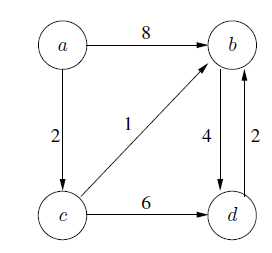
\includegraphics[scale=0.8]{bild1.png}
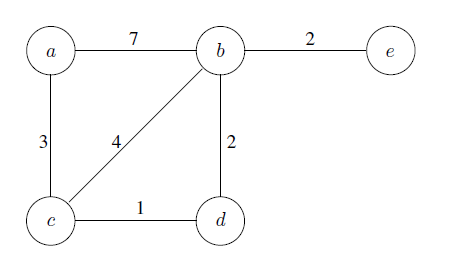
\includegraphics[scale=0.8]{bild2.png} 
\end{frame}

%---
\begin{frame}[fragile]

Mit Graphen k�nnen bin�re Beziehungen zwischen Objekten modelliert werden. Die Objekte werden
durch die Knoten, die Beziehungen durch die Kanten modelliert. \pause

1. Orte  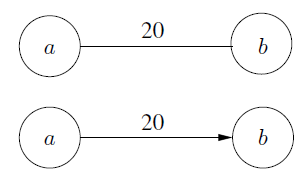
\includegraphics[scale=0.5]{bild3.png} ~~\pause Entfernungen, Kosten, Dauer \pause 

2. Personen 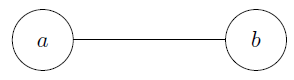
\includegraphics[scale=0.5]{bild4.png} ~~\pause ist verheiratet mit \pause 

3. Ereignisse 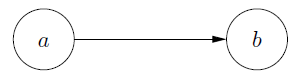
\includegraphics[scale=0.5]{bild5.png} ~~\pause a muss vor b geschehen

\end{frame}

%---
\begin{frame}[fragile]
Begriffe

\begin{minipage}{4cm}
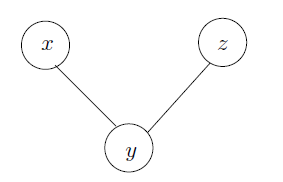
\includegraphics[scale=0.6]{bild6.png} \pause
\end{minipage}
\begin{minipage}{7cm}
x ist zu y adjazent, \\ \pause x und y sind Nachbarn, \\\pause x und z sind unabh�ngig, \\ \pause der Grad von y ist 2
\end{minipage} \pause

\begin{minipage}{4cm}
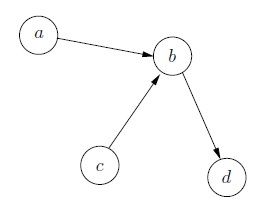
\includegraphics[scale=0.6]{bild7.png} \pause
\end{minipage}
\begin{minipage}{7cm}
a ist Vorg�nger von b, \\ \pause b ist Nachfolger von a, \\\pause Eingangsgrad von b ist 2, \\ \pause  Ausgangsgrad von b ist 1
\end{minipage} \pause

Ein \textit{Weg} ist eine Folge von adjazenten Knoten. \pause 

Ein \textit{Kreis} ist eine Weg, der zur�ck zum Startknoten f�hrt.
\end{frame}

\begin{frame}[fragile]
Implementation eine ungewichteten Graphen durch eine \textit{Adjazenzmatrix} 

\begin{minipage}{4cm}
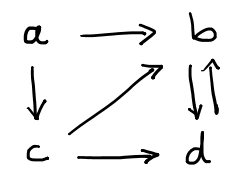
\includegraphics[scale=0.6]{bild20.png} 
\end{minipage}
\begin{minipage}{7cm} \pause
Wir ordnen jedem Knoten einen Index zu:
\\ \\
\begin{tabular}{|c|c|c|c|c|}
\hline Index & 0 & 1 & 2 & 3 \\
\hline Knoten  & a & b & c & d  \\
\hline
\end{tabular}
\end{minipage} \pause


\begin{minipage}{5cm}
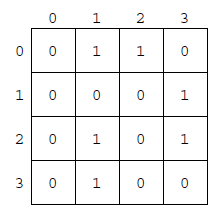
\includegraphics[scale=0.5]{bild8.png} 
\end{minipage} \pause
\begin{minipage}{5cm}
\begin{lstlisting} 
G = [[0, 1, 1, 0],  
     [0, 0, 0, 1],  
     [0, 1, 0, 1],  
     [0, 1, 0, 0]]
\end{lstlisting}  $\pause$
\end{minipage}
\begin{lstlisting} 
# gibt es Kante von a nach b? $\pause$
>>> G[0][1] $==$ 1  
True     
# alle Nachbarn von a  $\pause$
>>> for k in [j for j in range(len(G)) if G[0][j] $==$ 1]:
             print(k)             
1
2
>>> 
\end{lstlisting}
\end{frame}

\begin{frame}[fragile]
Implementation eines gewichteten Graphen durch eine \textit{Adjazenzmatrix} 
\begin{minipage}{4cm}
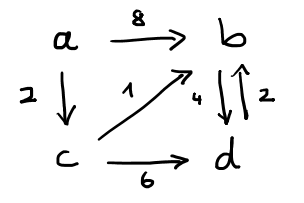
\includegraphics[scale=0.6]{bild21.png} 
\end{minipage}
\begin{minipage}{7cm} \pause
Wir ordnen jedem Knoten einen Index zu:
\\ \\
\begin{tabular}{|c|c|c|c|c|}
\hline Index & 0 & 1 & 2 & 3 \\
\hline Knoten  & a & b & c & d  \\
\hline
\end{tabular}
\end{minipage} \pause

Nicht vorhandene Kanten haben Kosten: \pause unendlich \pause

\begin{lstlisting} 
inf = float('inf') 
G = [[0,   8,   2, inf],  
     [inf, 0, inf,   4],  
     [inf, 1,   0,   6],  
     [inf, 2, inf,   0]]

# Kosten von von a nach b $\pause$
>>> G[0][1]
8
# alle Nachbarn von a  $\pause$
>>> for k in [j for j in range(len(G)) if j!=0 and G[0][j] < inf]:
		print(k)      
1
2
\end{lstlisting}


\end{frame}
\begin{frame}[fragile]
Analyse Implementation durch Adjazenzmatrizen: \pause

Platzbedarf = $O(|V|^2)$.\\ \pause
Direkter Zugriff auf Kante $(i,j)$ in konstanter Zeit m�glich. \\ \pause
Kein effizientes Verarbeiten der Nachbarn eines Knotens. \\ \pause
Sinnvoll bei dicht besetzten Graphen, d.h. Graphen mit quadratisch vielen Kanten. \\ \pause
Sinnvoll bei Algorithmen, die wahlfreien Zugriff auf eine Kante ben�tigen.

\end{frame}

\begin{frame}[fragile]
Implementation durch eines ungewichteten Graphen durch Adjazenzlisten, hier: Adjazenzmengen. 
Jedem Knoten wird in einem dictionary die Menge der Zielknoten der von ihm ausgehenden Kanten zugeordnet.
 
\begin{minipage}{5cm}
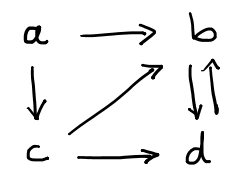
\includegraphics[scale=0.6]{bild20.png} 
\end{minipage} \pause
\begin{minipage}{5cm}
\begin{lstlisting} 
G = {'a':set('bc'),
     'b':set('d'), 
     'c':set('bd'),
     'd':set('b')}
\end{lstlisting}
\end{minipage} \pause

\begin{lstlisting} 
# gibt es Kante von a nach b  $\pause$
>>> 'b' in G['a']
True
# alle Nachbarn von a:  $\pause$
>>> for v in G['a']:
	print(v)
c
b
# alle Knoten von G durchlaufen: $\pause$
>>> for v in G:
       ....
\end{lstlisting}
\end{frame}

\begin{frame}[fragile]
Implementation eines gewichteten Graphen durch ein dictionary von dictionaries. Jedem Knoten wird ein dictionary zugeordnet, die jeder ausgehenden Kante ihre Kosten zuordnet.
 
\begin{minipage}{5cm}
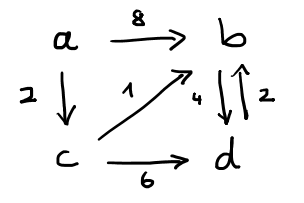
\includegraphics[scale=0.6]{bild21.png} 
\end{minipage} \pause
\begin{minipage}{5cm}
\begin{lstlisting} 
G = {'a': {'b':8, 'c':2},          
     'b': {'d':4},               
     'c': {'b':1, 'd':6},          
     'd': {'b':2}}
\end{lstlisting}
\end{minipage} \pause

\begin{lstlisting} 
 # gibt es Kante von a nach b  $\pause$
>>> 'b' in G['a']  
# die Kosten der Kante von a nach b:  $\pause$
>>> G['a']['b']     
# alle Nachbarn von a $\pause$
>>> for v in G['a']:   ....
# alle Knoten von G durchlaufen:  $\pause$
>>> for v in G:  ....

\end{lstlisting}
\end{frame}

\begin{frame}[fragile]

Analyse Implementation durch Adjazenzlisten: \pause

Platzbedarf = $O(|E|)$.\\ \pause
Bei Verwendung von Listen kein effizienter Zugriff auf Kante  $(x,y)$ m�glich. \\ \pause
Sinnvoll bei d�nn besetzten Graphen, d.h. Graphen mit nur linear vielen Kanten. \\ \pause
Sinnvoll bei Algorithmen, die, gegeben ein Knoten x, dessen Nachbarn verarbeiten m�ssen.

\end{frame}

\begin{frame}[fragile]
Der \textit{Floyd-Warshall Algorithmus} l�st das \textit{all-pairs-shortest-path} Problem. \pause Die Matrix
$D^k$ enth�lt die Kosten der k�rzesten Wege zwischen zwei Knoten $i$ und $j$, die als Zwischenknoten
nur die Knoten $0,1,..., k$ verwenden. \pause Dann l�sst sich $d_{i,j}^{k}$ errechnen durch das Minimum von 
 $d_{i,j}^{k-1}$ und  $d_{i,k}^{k-1} +  d_{k,j}^{k-1}$.

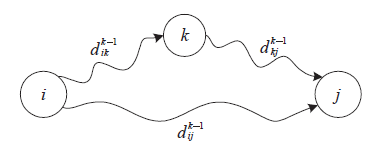
\includegraphics[scale=0.6]{bild12.png} \pause

Um die Kantenfolge zu rekonstruieren, wird gleichzeitig eine Folge von Matrizen $P^k$ aufgebaut, die an Position 
$p_{i,j}^{k}$ den vorletzten Knoten auf dem k�rzesten Weg von i nach j notiert, der nur �ber die Zwischenknoten 
$0,1,..., k$ l�uft.
\end{frame}

\begin{frame}[fragile]
\begin{lstlisting} 
def floyd (c):
    n = len(c)
    d = [[0]*n for j in range(n)]
    p = [[0]*n for j in range(n)]    
    for i in range(n):
        for j in range(n):
            d[i][j] = c[i][j]
            p[i][j] = i
    
    for k in range(n):
        for i in range(n):
            for j in range(n):
                tmp = d[i][k] + d[k][j]
                if tmp < d[i][j]:
                    d[i][j] = tmp
                    p[i][j] = p[k][j]
    return d, p

def printPath(p, i, j):
    if i $==$ j: print(i,end='')
    else:
        printPath(p,i,p[i][j])
        print(' - ' + str(j),end='')
\end{lstlisting}
\end{frame}


 \end{document}